\pagelayout{wide}
\setchapterstyle{kao}
\chapter{Résultats}

% Figure setup for
\captionsetup[figure]{format=plain,singlelinecheck=true,justification=centering}
\captionsetup[subfigure]{format=plain,singlelinecheck=true,justification=centering}

\todo[inline]{TODO : rédiger}

L'analyse du graphe de Software Heritage a permis de déterminer les quatre variables de recherche pour $TODO$
projets distincts dont les historique de développement sont eux aussi entièrement distincts deux à deux (aucun
projet analysé n'est un \en{fork} d'un autre).

Un aperçu initial des données collectées (figure~\ref{fig:data_description}) révèle quelques propriétés
intéressantes de la population étudiée. Les projets possédant des instructions de contribution ($TODO$, soit
$TODO\%$ des projets) sont significativement moins nombreux que ceux n'en possédant pas. L'écart entre la
moyenne et la médiane du nombre de \englpl{commit} récents, ainsi que sont écart type, indiquent une forte
variation de ce nombre au sein de la population étudiée, mais aussi la présence de quelques individus
extrêmes, avec un maximum à TODO \englpl{commit} récents observés dans un seul projet. Cette dernière
observation se retrouve aussi dans le nombre de \emph{contributeurs} récents, bien que de façon moins
spectaculaire. Rappelons à la vue des quantiles de cette dernière valeur que les projets ayant vu moins de
deux contributeurs distincts récents ont été exclus de l'étude (voir section
\ref{sec:constitution_echantillon} p.~\pageref{sec:constitution_echantillon}).

\begin{figure}
    \centering
    \begin{tabular}{cc}
        \begin{tabular}{ll}
 & hasContrib \\
count & 27619 \\
unique & 2 \\
top & no \\
freq & 23740 \\
\end{tabular}
 &
        \begin{tabular}{lr}
 & \textbf{recentCommitCount} \\
count & 60966.00 \\
mean & 61.79 \\
std & 408.96 \\
min & 2.00 \\
25\% & 8.00 \\
50\% & 19.00 \\
75\% & 49.00 \\
max & 36176.00 \\
\end{tabular}

        \\
        \begin{tabular}{lr}
 & \textbf{recentContributorCount} \\
count & 60966.000000 \\
mean & 3.246268 \\
std & 6.983897 \\
min & 2.000000 \\
25\% & 2.000000 \\
50\% & 2.000000 \\
75\% & 3.000000 \\
max & 688.000000 \\
\end{tabular}
 &
        \begin{tabular}{lr}
 & newContributorCount \\
count & 60966.000000 \\
mean & 0.522209 \\
std & 1.663200 \\
min & 0.000000 \\
25\% & 0.000000 \\
50\% & 0.000000 \\
75\% & 1.000000 \\
max & 130.000000 \\
\end{tabular}

    \end{tabular}

    \caption{Aperçu statistique des données collectées}
    \label{fig:data_description}
\end{figure}

\begin{figure}
    \begin{subfigure}[t]{0.5\textwidth}
        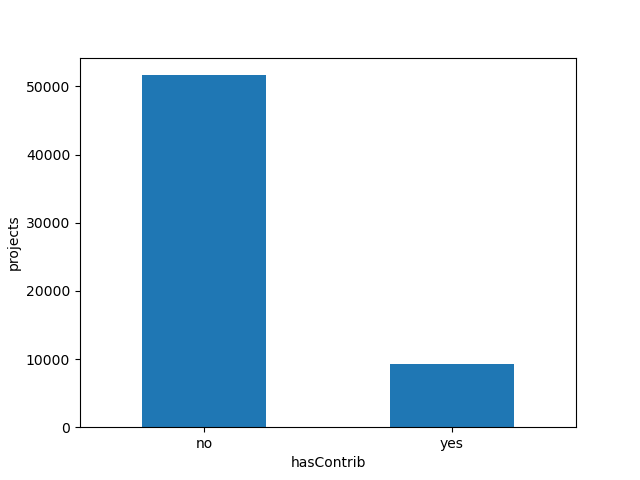
\includegraphics[width=\textwidth]{experiment/data_analysis/hasContrib_Count}
        \caption{Nombre de projets avec ou sans\\instructions de contribution}
    \end{subfigure}%
    \begin{subfigure}[t]{0.5\textwidth}
        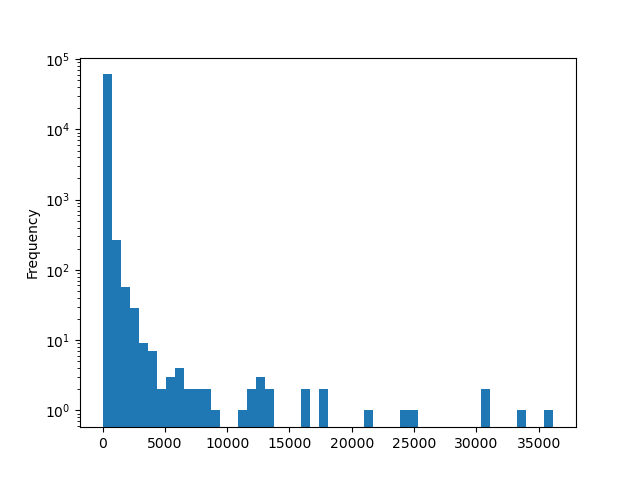
\includegraphics[width=\textwidth]{experiment/data_analysis/recentCommitCount_distribution}
        \caption{Nombre de \englpl{commit} récents\\(ordonnées logarithmiques)}
    \end{subfigure}

    \begin{subfigure}[t]{0.5\textwidth}
        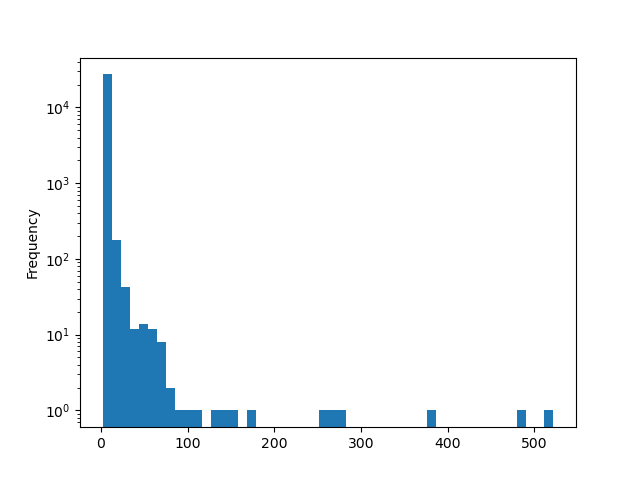
\includegraphics[width=\textwidth]{experiment/data_analysis/recentContributorCount_distribution}
        \caption{Nombre de contributeurs récents\\(ordonnées logarithmiques)}
    \end{subfigure}%
    \begin{subfigure}[t]{0.5\textwidth}
        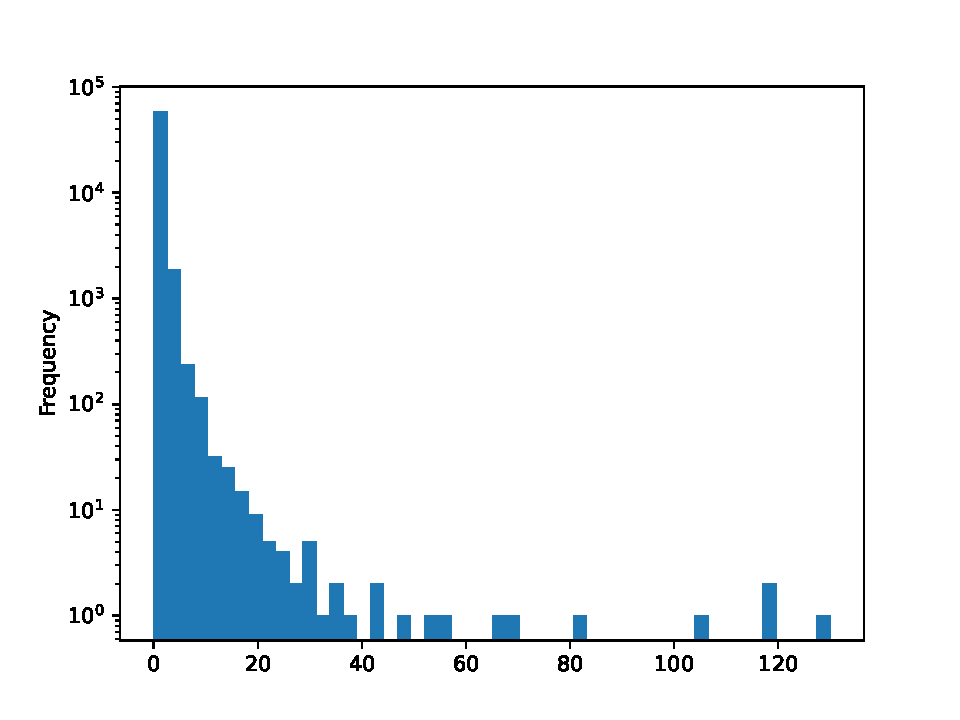
\includegraphics[width=\textwidth]{experiment/data_analysis/newContributorCount_distribution}
        \caption{Nombre de nouveaux contributeurs\\(ordonnées logarithmiques)}
    \end{subfigure}

    \caption{Distribution des individus selon chaque variable numérique}
    \label{fig:distribution}
\end{figure}

\begin{figure}
    \begin{subfigure}[t]{0.8\textwidth}
        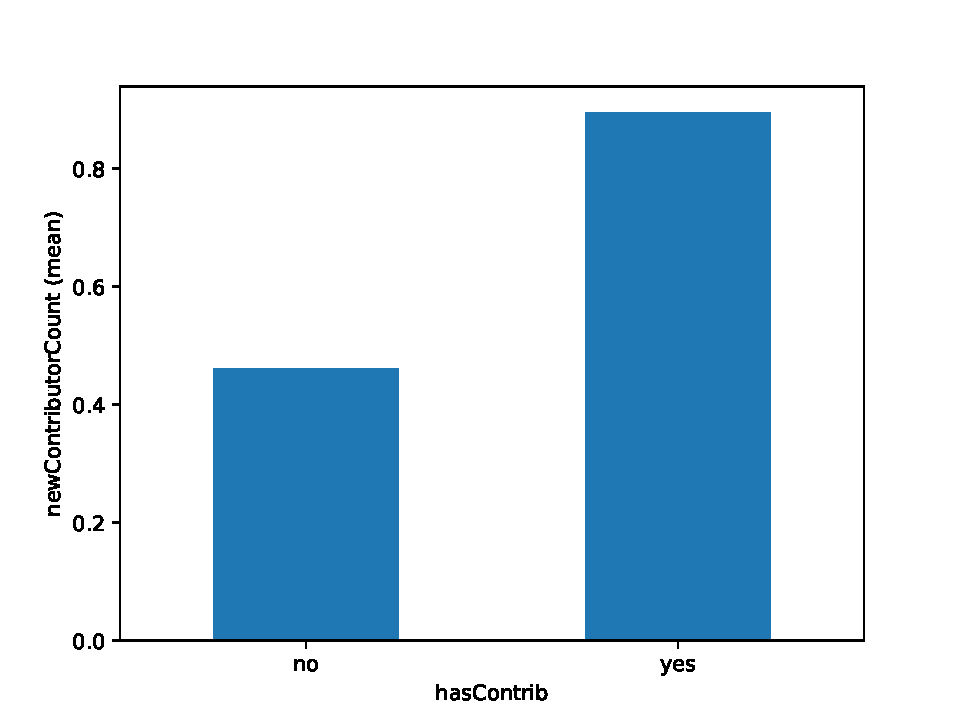
\includegraphics[width=\textwidth]{experiment/data_analysis/hasContrib_meanNewContributorCount}
        \caption{Moyenne du nombre de nouveaux contributeurs pour chaque catégorie}
    \end{subfigure}

    Mann-Whitney statistic: $U = 52115090$ ($p = 1.783731 \times 10^{-60}$, $ρ = 0.56593036$)
    \caption{Effet de la présence d'instructions de contribution}
    \label{fig:hasContrib}
\end{figure}

Ces deux catégories de projets ont été comparées avec le test de Mann-Whitney. Celui-ci donne une valeur $U =
TODO$ avec une taille d'effet $ρ = TODO$, ce qui signifie en langage courant que si l'on choisi au hasard un
projet $A$ possédant des instructions de contribution et un projet $B$ n'en possédant pas, il y a environ
$TODO\%$ de chances que le projet $A$ ait vu un plus grand nombre de nouveaux contributeurs durant la période
étudiée que le projet $B$. Le test confirme en outre avec un degré de confiance supérieur à $TODO\%$ ($p <
TODO$) que la distribution des valeurs au sein de ces deux catégories (projets avec instructions de
contribution ou sans) est bien différente, avec un avantage pour les projets avec instructions de
contribution.

\begin{figure}[ht]
    \centering
    \begin{subfigure}[t]{0.8\textwidth}
        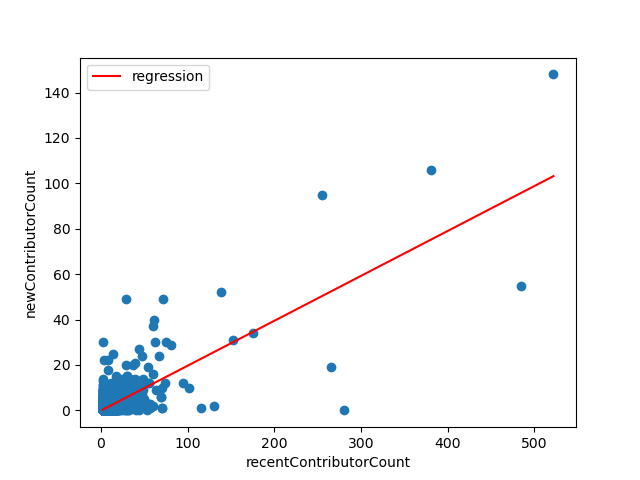
\includegraphics[width=\textwidth]{experiment/data_analysis/recentContributorCountRegression_linearScale}
        \caption{Échelle linéaire}
    \end{subfigure}

    \begin{subfigure}[t]{0.8\textwidth}
        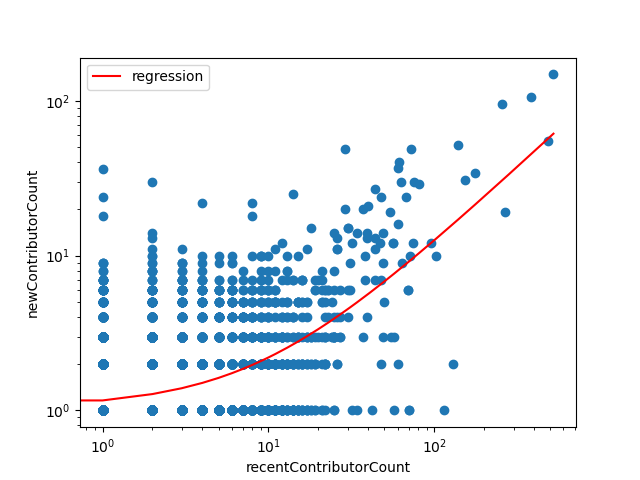
\includegraphics[width=\textwidth]{experiment/data_analysis/recentContributorCountRegression_logScale}
        \caption{Échelle logarithmique}
    \end{subfigure}

    $\mathit{newContributorCount} = \mathit{recentContributorCount} * 0.11540180 + 1.04427117$\\($r^2 = 0.28318792$)
    \caption{Nombre de nouveaux contributeurs en fonction du nombre de contributeurs récents uniques}
    \label{fig:contributorCount}
\end{figure}

\begin{figure}[ht]
    \centering
    \begin{subfigure}[t]{0.5\textwidth}
        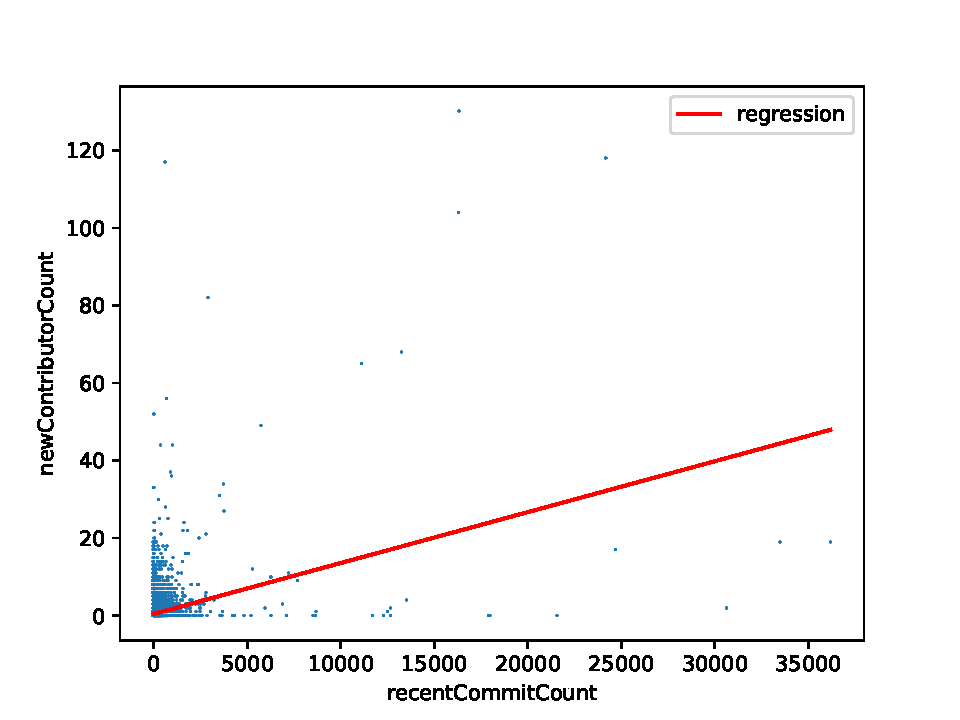
\includegraphics[width=\textwidth]{experiment/data_analysis/recentCommitCountRegression_linearScale}
        \caption{Échelle linéaire}
    \end{subfigure}%
    \begin{subfigure}[t]{0.5\textwidth}
        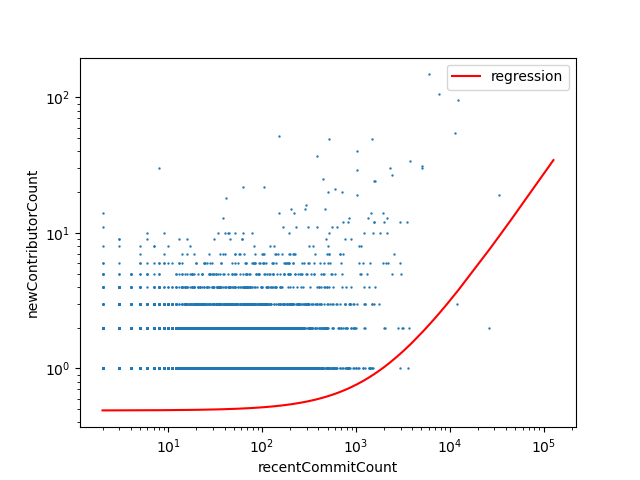
\includegraphics[width=\textwidth]{experiment/data_analysis/recentCommitCountRegression_logScale}
        \caption{Échelle logarithmique}
    \end{subfigure}

    $\mathit{newContributorCount} = \mathit{recentCommitCount} \times 0.00026672041 + 0.48979364$\\($r^2 = 0.12749825$)
    \caption{Nombre de nouveaux contributeurs en fonction du nombre de \englpl{commit} récents}
    \label{fig:commitCount}
\end{figure}

\pagelayout{margin}
